%%%%%%%%%%%%%%%%%%%%%%%%%%%%%%%%%%%%%%%%%
% Beamer Presentation
% LaTeX Template
% Version 1.0 (10/11/12)
%
% This template has been downloaded from:
% http://www.LaTeXTemplates.com
%
% License:
% CC BY-NC-SA 3.0 (http://creativecommons.org/licenses/by-nc-sa/3.0/)
%
%%%%%%%%%%%%%%%%%%%%%%%%%%%%%%%%%%%%%%%%%

%----------------------------------------------------------------------------------------
%	PACKAGES AND THEMES
%----------------------------------------------------------------------------------------

\documentclass[aspectratio=149]{beamer}
\usefonttheme[onlymath]{serif}


\mode<presentation> {

% The Beamer class comes with a number of default slide themes
% which change the colors and layouts of slides. Below this is a list
% of all the themes, uncomment each in turn to see what they look like.

\usetheme{default}
%\usetheme{AnnArbor}
%\usetheme{Antibes}
%\usetheme{Bergen}
%\usetheme{Berkeley}
%\usetheme{Berlin}
%\usetheme{Boadilla}
%\usetheme{CambridgeUS}
%\usetheme{Copenhagen}
%\usetheme{Darmstadt}
%\usetheme{Dresden}
%\usetheme{Frankfurt}
%\usetheme{Goettingen}
%\usetheme{Hannover}
%\usetheme{Ilmenau}
%\usetheme{JuanLesPins}
%\usetheme{Luebeck}
%\usetheme{Malmoe}
%\usetheme{Marburg}
%\usetheme{Montpellier}
%\usetheme{PaloAlto}
%\usetheme{Pittsburgh}
%\usetheme{Rochester}
%\usetheme{Singapore}
%\usetheme{Szeged}
%\usetheme{Warsaw}

% As well as themes, the Beamer class has a number of color themes
% for any slide theme. Uncomment each of these in turn to see how it
% changes the colors of your current slide theme.

%\usecolortheme{albatross}
\usecolortheme{beaver}
%\usecolortheme{beetle}
%\usecolortheme{crane}
%\usecolortheme{dolphin}
%\usecolortheme{dove}
%\usecolortheme{fly}
%\usecolortheme{lily}
%\usecolortheme{orchid}
%\usecolortheme{rose}
%\usecolortheme{seagull}
%\usecolortheme{seahorse}
%\usecolortheme{whale}
%\usecolortheme{wolverine}

%\setbeamertemplate{footline} % To remove the footer line in all slides uncomment this line
%\setbeamertemplate{footline}[page number] % To replace the footer line in all slides with a simple slide count uncomment this line

%\setbeamertemplate{navigation symbols}{} % To remove the navigation symbols from the bottom of all slides uncomment this line
}

\usepackage{graphicx} % Allows including images
\usepackage{booktabs} % Allows the use of \toprule, \midrule and \bottomrule in tables
\usepackage{verbatim}

\usepackage{mathtools} 
\usepackage{amssymb}
\usepackage{mathrsfs}
\usepackage{amsmath}
\usepackage{bm}

\usepackage{ragged2e}
\usepackage{etoolbox}
\usepackage{lipsum}

\usepackage{siunitx,booktabs}
\usepackage{pifont}
\usepackage{array}



\setbeamertemplate{enumerate items}[circle]
\usepackage{tikz}

\newcommand\mynum[1]{
  \usebeamercolor{enumerate item}
  \tikzset{beameritem/.style={circle,inner sep=0,minimum size=2ex,text=enumerate item.bg,fill=enumerate item.fg,font=\footnotesize}}%
  \tikz[baseline=(n.base)]\node(n)[beameritem]{#1};
}

\newcommand\mynumm[1]{
  \usebeamercolor{enumerate item}
  \tikzset{beameritem/.style={rectangle,inner sep=0,minimum size=2ex,text=enumerate item.bg,fill=enumerate item.fg,font=\footnotesize}}%
  \tikz[baseline=(n.base)]\node(n)[beameritem]{#1};
}

\def\Put(#1,#2)#3{\leavevmode\makebox(0,0){\put(#1,#2){#3}}}

\setbeamertemplate{footline}[frame number]

%----------------------------------------------------------------------------------------
%	TITLE PAGE
%----------------------------------------------------------------------------------------

\title{ Subsidized Housing with Slum Externalities: \\ Evidence from South Africa } % The short title appears at the bottom of every slide, the full title is only on the title page

\author{Stefano Polloni \\
joint with Ben Bradlow and Will Violette} 

 % Your institution as it will appear on the bottom of every slide, may be shorthand to save space

\date{February 2017} %\today} % Date, can be changed to a custom date

\begin{document}

\beamertemplatenavigationsymbolsempty

\begin{frame}
\titlepage % Print the title page as the first slide
\end{frame}

%\begin{frame}
%\frametitle{Overview} % Table of contents slide, comment this block out to remove it
%\tableofcontents % Throughout your presentation, if you choose to use \section{} and \subsection{} commands, these will automatically be printed on this slide as an overview of your presentation
%\end{frame}

%----------------------------------------------------------------------------------------
%	PRESENTATION SLIDES
%----------------------------------------------------------------------------------------
\section{Introduction}
%------------------------------------------------

\begin{frame}
\frametitle{Context}

\begin{itemize}
\item Rapid Urbanization in the developping world during past decades.
\vspace{1mm}
\item Significant portion of low-income city-dwellers live in slums, i.e. unserviced and temporary/informal housing structures.
\vspace{1mm}
\item Disagreement on whether slum-dwellers are in a transitory phase (Glaeser, 2011) or stuck in proverty traps (Marx, 2013). 
\vspace{1mm}
\item Regardless, slum living conditions are poor:
\vspace{1mm}
\begin{itemize}
\item inadequate living space
\item poor sanitation and water access
\item high crime levels
\item low public goods provision


\end{itemize}
\vspace{1mm}
\end{itemize}

\end{frame}

%------------------------------------------------

\begin{frame}
\frametitle{Motivation}

Why should Governments intervene? 

\begin{enumerate}
\item Redistributive goals. 
\vspace{1mm}
\item Slum Externalities:
  \begin{itemize}
    \item increased fire hazards, health risks, crime.
    \item overburdening of public infrastructure, e.g. water and sewage.

  \end{itemize}
\end{enumerate}

\vspace{2mm}

Standard policy portfolio:



\begin{itemize}
\item Altering property rights and land regulations.
\vspace{1mm}
\item On-site slum upgrading/servicing. 
\vspace{1mm}
\item Subsidized formal housing. 
\end{itemize}
\vspace{1mm}

\end{frame}

%------------------------------------------------

\begin{frame}
\frametitle{This Paper:}

\begin{itemize}
\item Focus on subsidized formal housing.
\vspace{1mm}
\item Learn from the South African experience with post-apartheid Reconstruction and Development Programme (RDP).
\vspace{1mm}
\item Treat subsidized housing as a place-based policy that affects surrounding neighborhoods and households' location decision.
\vspace{1mm}
\item Think about "optimal" housing subsidy if slums generate externalities.
\vspace{1mm}
\item Think about interactions between subsidized formal housing and informal housing:
\begin{itemize}
  \item Subsidized units may attract informal structures because of service access and available land. 
  \item "Back-yarding" a prevalent phenomena in South Africa.
\end{itemize}
\end{itemize}


\end{frame}

%------------------------------------------------

\begin{frame}
\frametitle{Research Questions}
  \begin{enumerate}
    \item What is the extent, if any, of slum externalities ?
  \vspace{1mm}
    \item Do formal housing subsidies spillover to informal housing?
  \vspace{1mm}
    \item Given {\!\!\!\mynum{1}} and {\!\!\!\mynum{2}}, what are the GE welfare impacts of subsidized formal housing?
  \end{enumerate}

Today:
\begin{itemize}
  \item Brief description of SA housing subsidies. 
  \item Description of available data.
  \item Some empirical evidence towards answering {\!\!\!\mynum{1}} and {\!\!\!\mynum{2}}.
  \item Outline of a model towards {\!\!\!\mynum{3}}.
\end{itemize}



\end{frame}


%------------------------------------------------

\begin{frame}
\frametitle{RDP housing in a nutshell }
  \begin{itemize}
    \item The RDP is a policy framework implemented in 1994 to address several socioeconomic issues under apartheid rule.
    \item Includes a large housing subsidy scheme, which provides eligible households the opportunity of owning their first house.
    \item Eligibility is based on citizenship, marital status and income.
    \item Program recipients receive a one-off capital subsidy (the house) at very low or no cost.
    \item Large excess demand; allocation process loosely regulated by various priority systems and wait lists, with many noted cases of corruption.
    \item Supply is planned by municipal and provincial housing agencies, construction is outsourced to private developers, with constraints on costs per unit, services access, and rooms/lot sizes.
  \end{itemize}



\end{frame}

%------------------------------------------------

\begin{frame}
\frametitle{Data Sources}
\vspace{-1em}
{\bf Three main data sources: }

\vspace{1em}

\begin{enumerate}
  \item Census data on households and individuals, 2 cross-sections.
  \item Data on buildings, 2-cross sections.
  \item Data on real-estate transactions.
\end{enumerate}

\end{frame}

%------------------------------------------------

\begin{frame}
\frametitle{Data Sources}
1. Census data:
\vspace{2mm}
  \begin{itemize}
    \item National coverage of the 2001 and 2011 census, at the respondent level. 

    \item Individuals and household geographically identified at the small area level ($\,\,\sim$ 170 households per small area)
    \vspace{2mm}
    \item  Basic information on demographics, employment, income, education and dwelling characteristics.

\end{itemize}
\end{frame}

%------------------------------------------------

\begin{frame}
\frametitle{Data Sources}
2. Building-Based Land use data:
\vspace{2mm}
  \begin{itemize}
    \item Exhaustive building census based on aerial imagery.
    \vspace{2mm}
    \item Building stock differentiable by various categories: residential, commercial, industrial, etc.
    \vspace{2mm}
    \item Within residential, ability to differentiate formal from informal housing, including backyard shacks.
    \vspace{2mm}
    \item 2 waves:
    \begin{itemize} 
      \item 2001 covering Gauteng Province and Cape-town metro area.
      \item 2012 National coverage.
    \end{itemize}
\end{itemize}
\end{frame}


%------------------------------------------------

\begin{frame}
\frametitle{Data Sources}
3. Deeds data:
\vspace{2mm}
  \begin{itemize}
    \item Universe of housing transactions recorded during 2002-2011 in all affordable areas\footnote{defined as census enumeration areas with mean house price value less than R500,000 in 2010.} in the country. ($\sim$\! 1.2M transactions)
    \vspace{2mm}
    \item Exact geographic location of traded property, but limited information on characteristics other than price and lot size.
    \vspace{2mm}
    \item RDP transactions noisily identifiable by filtering on Seller Name, price and lot size. ($\sim$\! 300K transactions)
\end{itemize}
\end{frame}

%------------------------------------------------

\begin{frame}
\frametitle{Using BBLU data to examine Formal/Informal housing response}

Formal Housing\footnote{grey polygons denote location of RDP projects}:

\vspace{4mm}

\begin{tabular}{cc}
 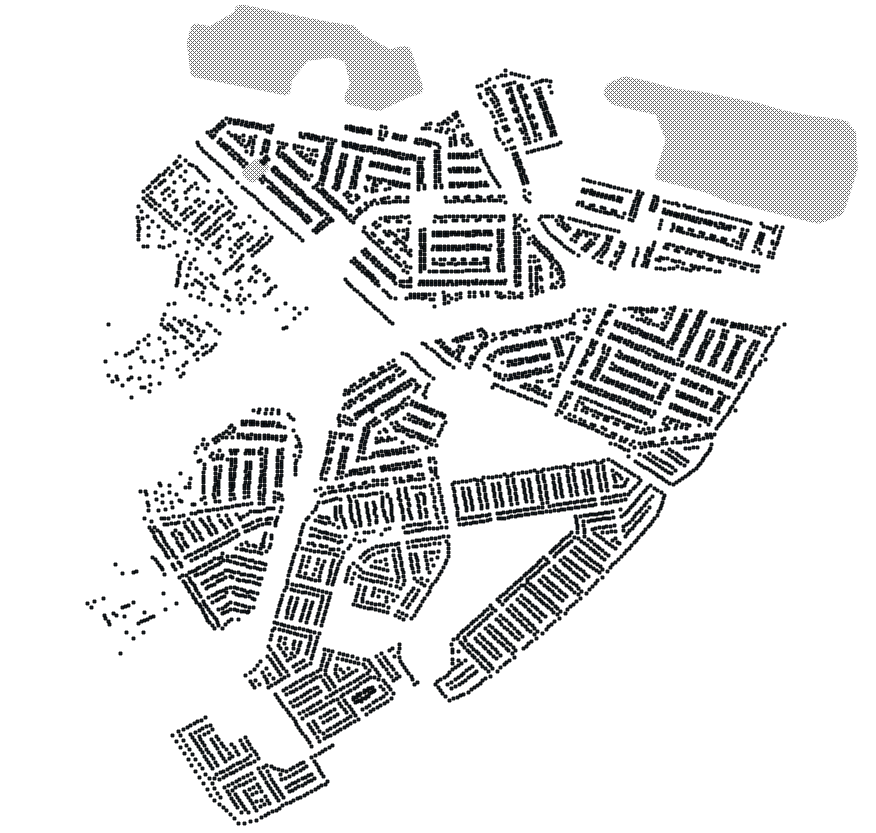
\includegraphics[scale=0.18]{pre_formal.png} & 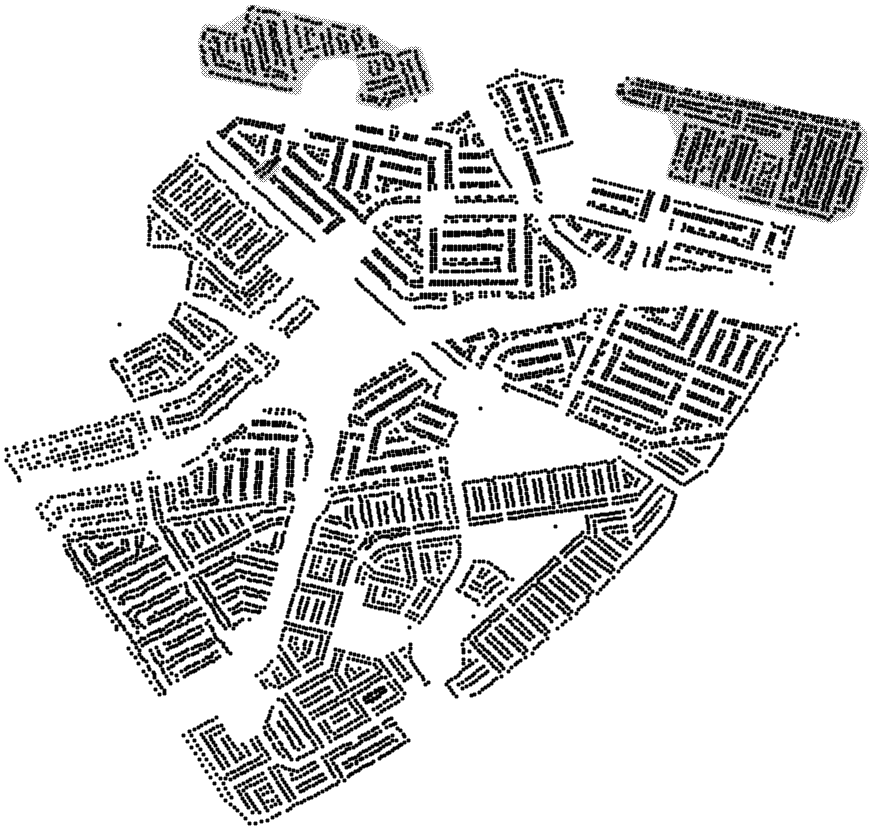
\includegraphics[scale=0.18]{post_formal.png} \\
  2001 & 2012 \\
\end{tabular}

\end{frame}

%------------------------------------------------

\begin{frame}
\frametitle{Using BBLU data to examine Formal and Informal housing}

Informal Housing\footnote{grey polygons denote location of RDP projects}:

\vspace{4mm}

\begin{tabular}{cc}
 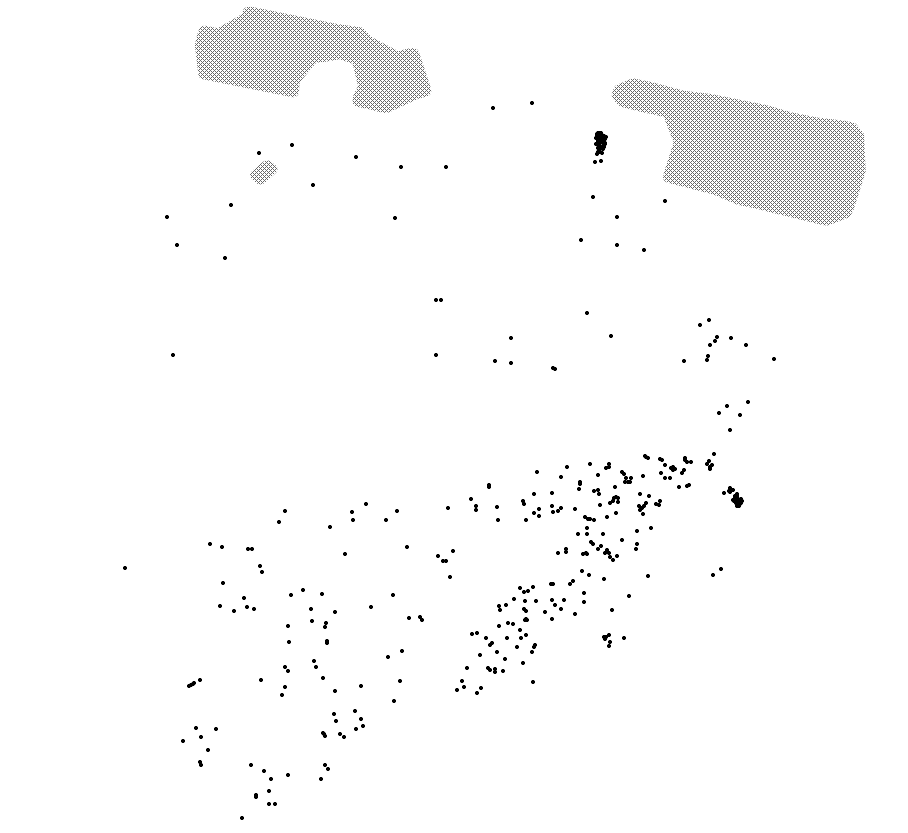
\includegraphics[scale=0.18]{pre_informal.png} & 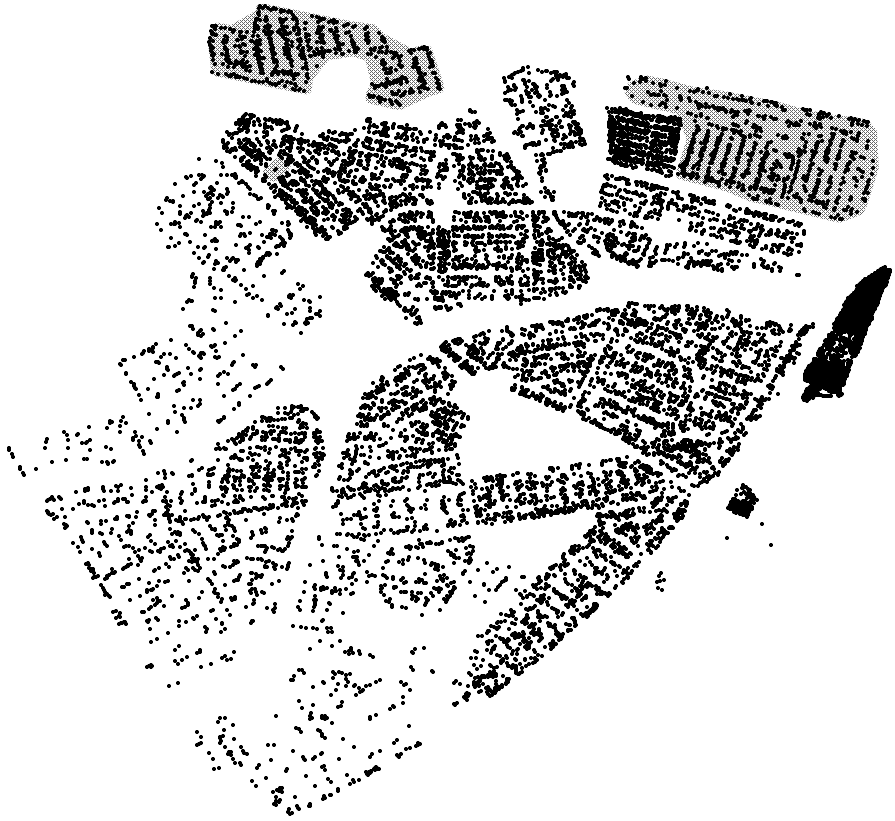
\includegraphics[scale=0.18]{post_informal.png} \\
  2001 & 2012 \\
\end{tabular}

\end{frame}

%------------------------------------------------

\begin{frame}
\frametitle{Using BBLU data to examine Formal and Informal housing}

Residential housing density (buildings per 1000m$^2$) using data from 94 RDP projects in Gauteng Province:

\vspace{3mm}
\begin{tabular}{rcc}
\begin{tabular}{rcc}
 & {\footnotesize Mean } & {\footnotesize S.D.} \\\hline
{\footnotesize 2001}\\
{\footnotesize Formal:} & {\footnotesize 0.34 }&{\footnotesize 0.54} \\
{\footnotesize Informal:} & {\footnotesize 0.84 }&{\footnotesize 1.02} \\
{\footnotesize 2012}\\
{\footnotesize Formal:} & {\footnotesize 1.91 }&{\footnotesize 0.67} \\
{\footnotesize Informal:} & {\footnotesize 1.70 }&{\footnotesize 1.61} 
\end{tabular}
& 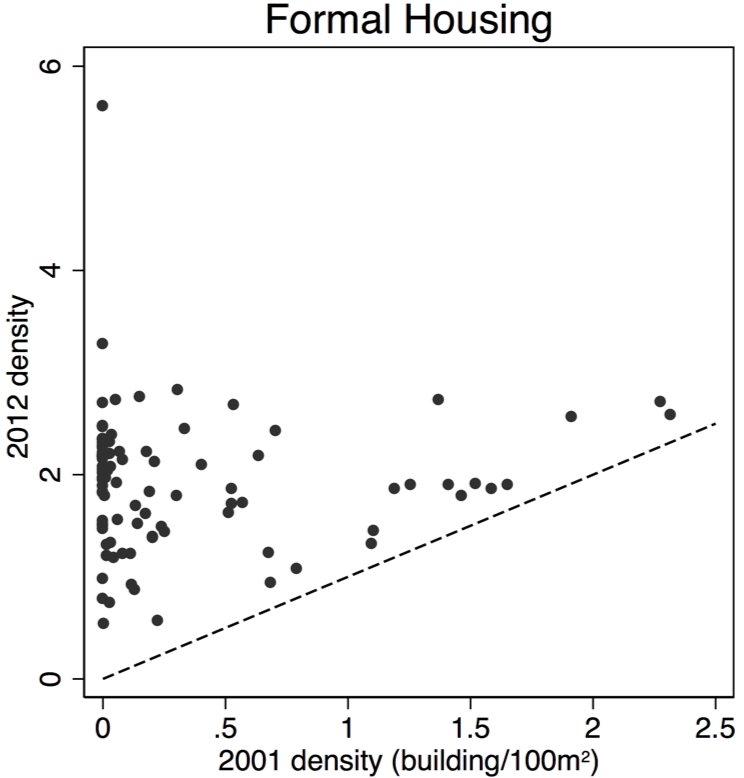
\includegraphics[scale=0.14]{formal.png} & 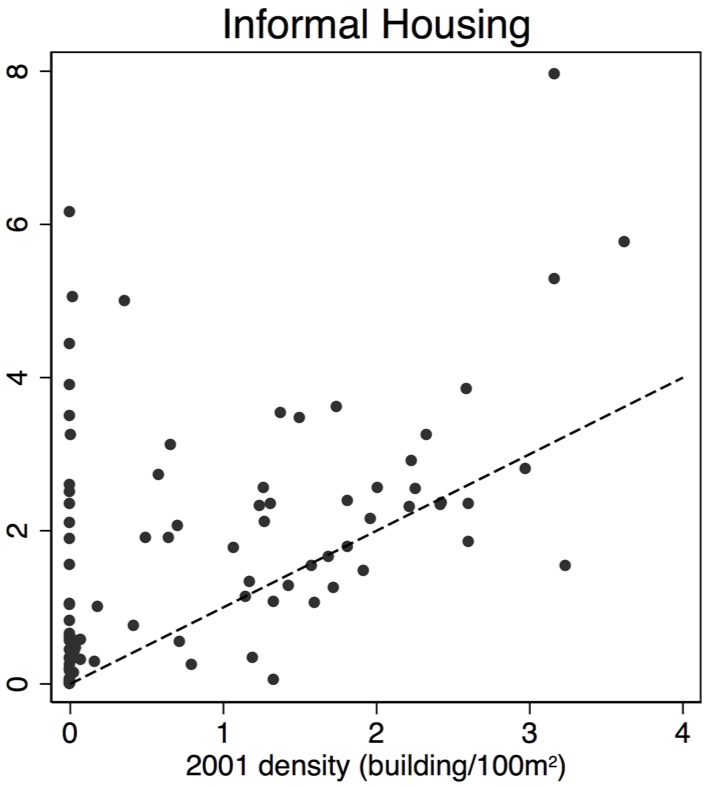
\includegraphics[scale=0.14]{informal.png}
\end{tabular}


\end{frame}
%------------------------------------------------

\begin{frame}
\frametitle{Using deeds data to estimate RDP impact on housing prices}

A first-pass DD aproach:
\begin{itemize}
  \item Identify areas where many clustered RDP houses were sold at similar dates.
  \item Examine house prices in adjacent areas, before and after construction, near and far from RDP project.
  \item Rely on spatial proximity for identification. 

\end{itemize}

\end{frame}

%------------------------------------------------

\begin{frame}
\frametitle{Using deeds data to estimate RDP impact on housing prices}

\begin{center}
\begin{figure}
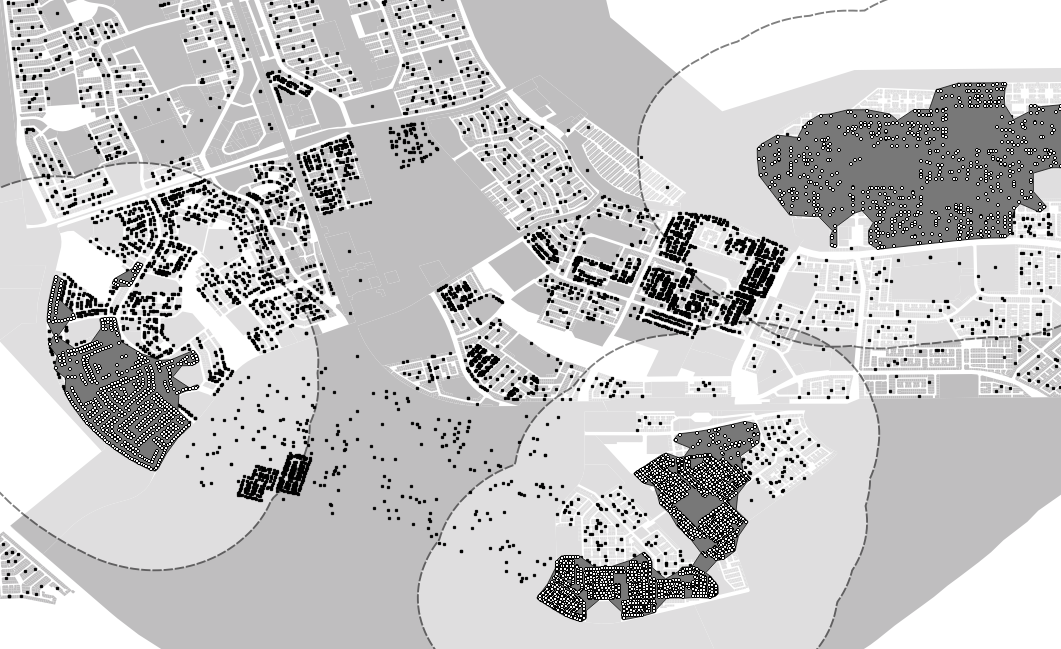
\includegraphics[scale=0.30]{design2.png}
\vspace{-3mm}
\end{figure}
\end{center}



\end{frame}

%------------------------------------------------

\begin{frame}
\frametitle{Using deeds data to estimate RDP impact on housing prices}

\begin{center}
\begin{figure}
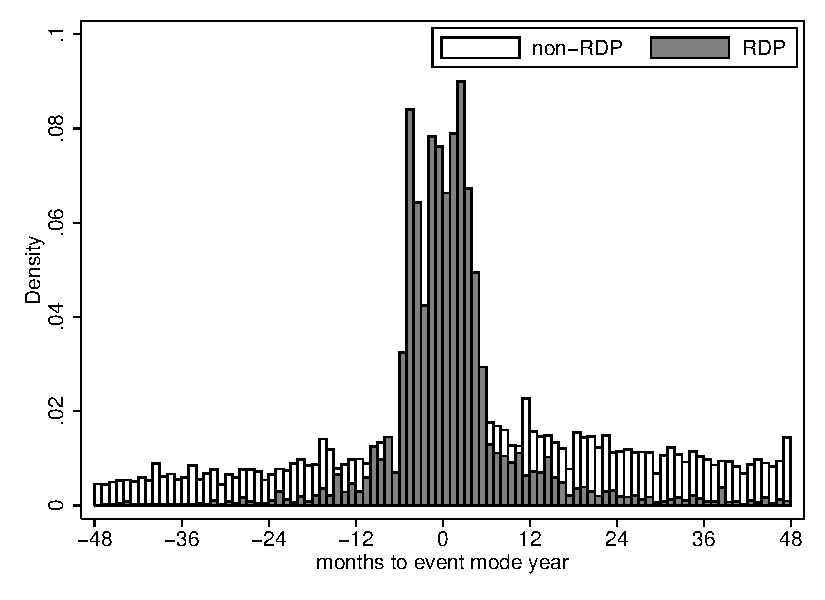
\includegraphics[scale=0.65]{summary_densitytime.pdf}
\vspace{-3mm}
\caption{density of RDP vs Non-Rdp transactions centered around "event month"}
\end{figure}
\end{center}


\end{frame}

%------------------------------------------------

\begin{frame}
\frametitle{Using deeds data to estimate RDP impact on housing prices}

\begin{center}
\begin{figure}
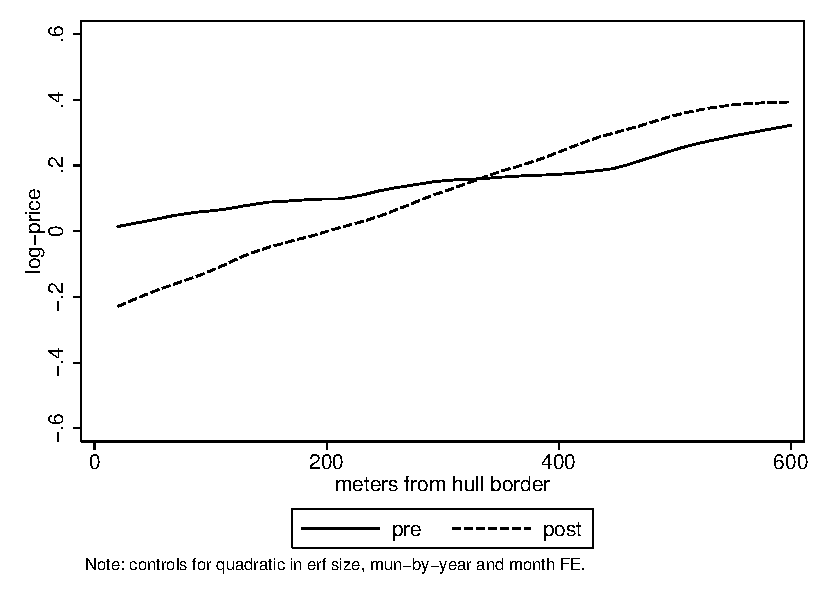
\includegraphics[scale=0.65]{reg_pm1.pdf}
\vspace{-3mm}
\caption{Smoothed distance dummy coefficients of log-price of Non-RDP transactions, before and after mode year of construction.}
\end{figure}
\end{center}


\end{frame}

%------------------------------------------------

\begin{frame}
\frametitle{Using deeds data to estimate RDP impact on housing prices}

\begin{center}
\begin{figure}
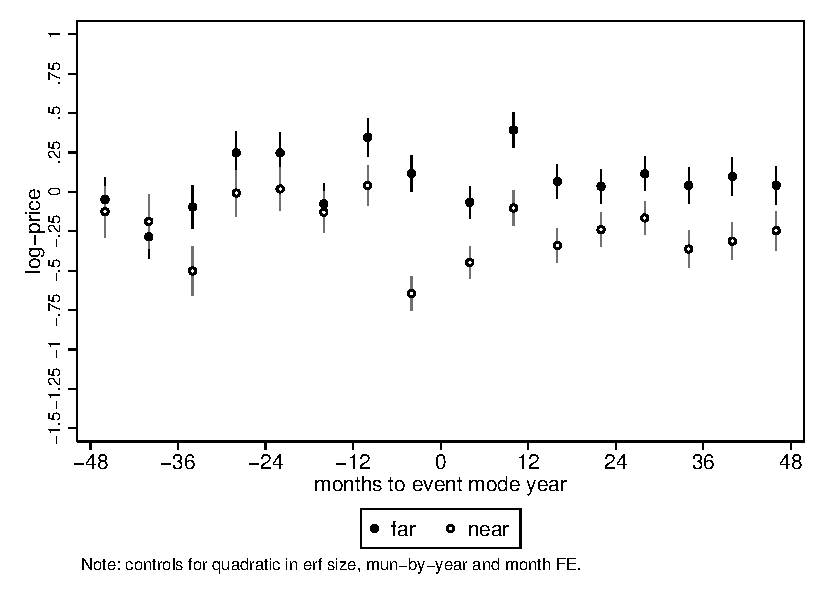
\includegraphics[scale=0.65]{timereg_pm1.pdf}
\vspace{-3mm}
\caption{6-month dummy coefficients of log-price of Non-RDP transactions, $<$300m (near) and $>$300m (far) from border of RDP project.}
\end{figure}
\end{center}


\end{frame}

%------------------------------------------------



\begin{frame}
\frametitle{A Model of Housing with Slum Externalities}

Basic Setup:
\vspace{2mm}
\begin{itemize}
  \item A city is comprised of $N$ residential neighborhoods indexed $n\in\{1,...,N\}$. 
  \vspace{2mm}
  \item Each neighborhood has a formal and informal housing sector, indexed $s\in\{F,I\}$.
  \vspace{2mm}
  \item All jobs are in the CBD and pay a fixed wage rate; commuting to the CBD is costly.
\end{itemize}


\end{frame}

%------------------------------------------------

\begin{frame}
\frametitle{Housing Demand}

Housing Demand:
\vspace{2mm}
\begin{itemize}
  \item Measure one of freely-mobile agents inelastically demand one unit of housing.
  \vspace{2mm}
  \item An agent $i$ has idiosyncratic tastes for neighborhoods, represented by the vector $\bm{\epsilon}_i \in \mathbb{R}^{2N}$ of neighborhood-sector specific valuations.
  \vspace{2mm}
  \item The distribution of preferences in the population is given by density $f(\bm{\epsilon})$ such that $\int f(\bm{\epsilon}) d\bm{\epsilon} = 1$.
\end{itemize}


\end{frame}

%------------------------------------------------

\begin{frame}
\frametitle{Housing Demand}

Indirect Utility:

\begin{equation*}
\begin{aligned}
u_{ins} \,& =\, A_n\,+\, B_s - R_{ns} \,+\, \epsilon_{ins} \\
        \,& =\, v_{ns} \,+\, \epsilon_{ins}
\end{aligned}
\end{equation*}

With:
\vspace{2mm}
\begin{itemize}
  \item $A_n$ is net-of-commuting and amenity-adjusted wage received in $n$.
  \item $B_s$ is a utility component specific to living in sector $s$
  \item $R_{ns}$ is the rental rate of housing.
  \item $\epsilon_{ins}$ is individual $i$'s taste for neighborhood-sector pair $(n,s)$.
\end{itemize}

\vspace{5mm}

Individual $i$ takes exogenous quantities $\{\bm{A},\bm{B},\bm{\epsilon}_i\}$ and endogenous rents $\bm{R}$ as given, and locates in pair $(n,s)$ yielding the highest indirect utility.


\end{frame}

%------------------------------------------------

\begin{frame}
\frametitle{Housing Demand}

Aggregate housing demand $H_{ns}$ in $(n,s)$ given by:

\begin{equation*}
\begin{aligned}
H_{ns} \,\,& =\,\, \int I\Big( \, u_{ins} \,=\, \max_{n's'}\{u_{in' s'} \,\,|\,\, \bm{A},\bm{B},\bm{R}\,\} \Big)f(\bm{\epsilon}) d\bm{\epsilon}    \\[.2em]
        \,\,& =\,\, D_{ns}(\bm{A},\bm{B},\bm{R})
\end{aligned}
\end{equation*}

\end{frame}

%------------------------------------------------

\begin{frame}
\frametitle{Housing Supply}

\begin{itemize}
  \item Neighborhoods are endowed with $L_n$ units of land.
  \item A share $\theta_{nF}$ of the total land stock is available for formal residential development, while the rest, $\theta_{nI} = 1-\theta_{nF}$, is vacant or public land suited for informal housing.
  \item Price-taking landlords supply housing by combining land and materials $M$ with CRS technology $q(L,M)$.
  \item Materials are supplied at fixed cost $c$ on a large national market.
  \item Government can subsidize housing in market $(n,s)$ at a rate of $\delta_{ns}$ per unit.
\end{itemize}

Because land is fixed in every market, the marginal cost of housing is increasing. The inverse supply curve in $(n,s)$ is:

\begin{equation*}
R_{ns} \,\, =\,\, S(H_{ns},\theta_{ns}L_n) - \delta_{ns}
\end{equation*} 

\vspace{4mm}

\end{frame}

%------------------------------------------------

\begin{frame}
\frametitle{Equilibrium}
{\small
Given density $f(\bm{\epsilon})$ and exogenous quantities $\{\bm{A},\bm{B},\bm{L},\bm{\theta}\}$, an equilibrium consists of rents $\bm{R}^*$ and housing quantities $\bm{H}^*$ such that all housing markets clear, that is, $\forall (n,h)$:

\begin{equation*}
\begin{aligned}
& H^*_{ns} \,\, =\,\, D_{ns}(\bm{A},\bm{B},\bm{R}^*) \\
\text{and}\quad & R^*_{ns} \,\, =\,\, S(H^*_{ns},\theta_{ns}L_n) - \delta_{ns} \text{,}
\end{aligned}
\end{equation*} }


\noindent and all agents live somewhere: $\sum_{n}\sum_{s} H^*_{ns} = 1$

\begin{center}
\begin{figure}
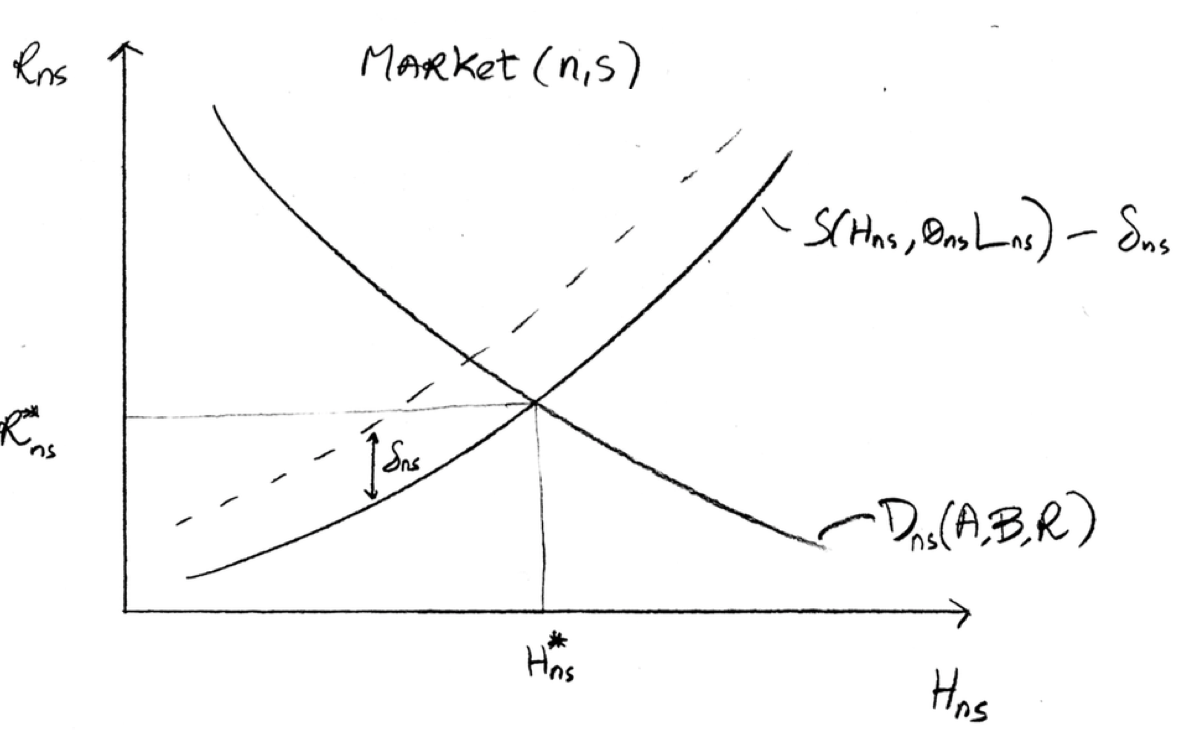
\includegraphics[scale=0.16]{market.png}
\vspace{-3mm}
\end{figure}
\end{center}


\end{frame}

%------------------------------------------------

\begin{frame}
\frametitle{Welfare}

The sum of individuals' utility is given by:

\begin{equation*}
U \,\, =\,\, \int \max_{n's'}\{u_{in' s'}\,\,|\,\, \bm{A},\bm{B},\bm{R}^*\,\}f(\bm{\epsilon}) d\bm{\epsilon} 
\end{equation*}

\vspace{3mm}

\noindent and total landlords' profit is:

\begin{equation*}
\Pi \,\, =\,\, \sum_{n}\sum_{s} \Bigg(\,\int_0^{H^*_{ns}} [R^*_{ns} - (S(x,\theta_{ns}L_n) - \delta_{ns})]dx \, \Bigg) 
\end{equation*} 

\vspace{3mm}

Total social welfare is:

\begin{equation*}
W = U + \Pi
\end{equation*} 

\end{frame}

%------------------------------------------------

\begin{frame}
\frametitle{Welfare Implications of Subsidies (No Market Failures)}

We are interested in the welfare implications of the government subsidizing formal housing in a subset $\mathcal{N}\subset\{1,...,N\}$ of neighborhoods:

\vspace{2mm}

\begin{equation*}
 \delta_{ns} = \begin{cases} 
      \,\,\delta & \text{if}\,\, n\in\mathcal{N} \,\,\text{and}\,\, $s=F$ \\
      \,\,0 & \text{otherwise} 
   \end{cases}
\end{equation*} 

\vspace{2mm}

After some algebra, we can show that the marginal welfare effect of changing $\delta$ simplifies to: 

\vspace{2mm}

\begin{equation*}
\frac{\partial W}{\partial\delta} \,\,=\,\, \frac{\partial U}{\partial\delta} \,\,+\,\, \frac{\partial \Pi}{\partial\delta} \,\,=\,\, \sum_{n\in\mathcal{N}} H^*_{nF}
\end{equation*} 


\end{frame}

%------------------------------------------------

\begin{frame}
\frametitle{Welfare Implications of Subsidies (No Market Failures)}

The total cost of the subsidy is given by $TC = \sum_n\sum_s H^*_{ns}\delta_{ns}$ and its marginal cost is therefore:
\begin{equation*}
 \frac{\partial TC}{\partial \delta} \,\,=\,\, \sum_{n\in\mathcal{N}} \Big( H^*_{nF} \,\,+\,\, \delta\frac{\partial H^*_{nF}}{\partial \delta} \Big)
 \end{equation*} 

 \vspace{1mm}

 The extra term in this expression relative to (2) represents the marginal deadweight loss from an increase in $\delta$. The magnitude of the inefficiencies depends on the population responses in subsidized markets, $\frac{\partial H^*_{nF}}{\partial \delta}$.

\end{frame}

%------------------------------------------------

\begin{frame}
\frametitle{Welfare Implications with Slum Externalities}

We consider an external utility cost from informal housing of the form:

\begin{equation*}
A_n \,\,=\,\, \bar{A}_n \,\,+\,\, a\Big(\frac{H_{nI}}{L_n}\Big)
\end{equation*} 


where $a'(.)<0$. The private decision of locating in $(n,I)$ negatively impacts all residents in $n$ because of congestion effects. The welfare response to $\delta$ is now:

\begin{equation*}
\frac{\partial W}{\partial\delta} \,\,=\,\, \sum_{n\in\mathcal{N}} H^*_{nF} \,\,+\,\, \sum_{n} \underbracket{a'\Big(\frac{H^*_{nI}}{L_n}\Big)}_{(<0)}\,\underbracket{\frac{\partial H^*_{nI}}{\partial \delta}}_{(<0)}\,\frac{(H^*_{nF}+H^*_{nI})}{L_n}
\end{equation*}

The subsidy $\delta$ makes formal housing in $\mathcal{N}$ more attractive relative to informal housing. Marginal residents moving to $\mathcal{N}$ make remaining residents better-off because of reduced congestion.

\end{frame}

%------------------------------------------------

\begin{frame}
\frametitle{Welfare Implications with Slum Externalities}

Since the cost of the subsidy is unaffected by the externality, the marginal deadweight loss is now:

\begin{equation*}
\begin{aligned}
MDWL \,\,&=\,\, \frac{\partial TC}{\partial \delta} - \frac{\partial W}{\partial \delta} \\[.6em]
     \,\,&=\,\, \sum_{n\in\mathcal{N}} \,\delta\frac{\partial H^*_{nF}}{\partial \delta} \,\,-\,\, \sum_{n} \, a'\Big(\frac{H^*_{nI}}{L_n}\Big)\,\frac{\partial H^*_{nI}}{\partial \delta}\,\frac{(H^*_{nF}+H^*_{nI})}{L_n} \\
\end{aligned}
\end{equation*}

 $\delta=0$ implies $MDWL<0$. Some level of subsidy $\delta$ is welfare improving when compared to no subsidy. This is expected since the social benefits exceed the private benefits of moving from informal to formal housing. 

\end{frame}


%------------------------------------------------

\begin{frame}
\frametitle{Welfare with Slum Externalities and Subsidy Spillovers.}

To capture the possibility of increased "backyarding", we now assume subsidies in the formal sector spillover to the informal sector at no additional cost for the government:

\begin{equation*}
 \delta_{ns} = \begin{cases} 
      \,\,\delta & \text{if}\,\, n\in\mathcal{N} \,\,\text{and}\,\, $s=F$ \\
      \,\,\alpha\delta & \text{if}\,\, n\in\mathcal{N} \,\,\text{and}\,\, $s=I$ \\
      \,\,0 & \text{otherwise} 
   \end{cases}
\end{equation*}

This yields:

\begin{equation*}
\frac{\partial W}{\partial\delta} \,\,=\,\, \sum_{n\in\mathcal{N}} \big( H^*_{nF} + \alpha H^*_{nI} \big)  \,\,+\,\, \sum_{n} \underbracket{a'\Big(\frac{H^*_{nI}}{L_n}\Big)}_{(<0)}\,\underbracket{\frac{\partial H^*_{nI}}{\partial \delta}}_{(\lessgtr0)}\,\Big(\frac{H^*_{nF}+H^*_{nI}}{L_n} \Big)
\end{equation*} 

\end{frame}


%------------------------------------------------

\begin{frame}
\frametitle{Welfare with Slum Externalities and Subsidy Spillovers.}

The presence of such spillovers alter welfare implications in two ways:

\begin{itemize}
  \item Suppliers of informal housing benefit from an increase in profit due to the indirect subsidies.
  \item For $n\in\mathcal{N}$, the sign of informal housing response $\frac{\partial H^*_{nI}}{\partial\delta}$ is now ambiguous and depends on the magnitude of $\alpha$.\footnote{ This can also be shown formally by combining the equilibrium conditions in (1) and using the implicit function theorem. For $n\in\mathcal{N}^C$, $\frac{\partial H^*_{nI}}{\partial\delta}$ remains unambiguously negative.} When $\alpha$ is large, the indirect subsidies in $(n,I)$ dominate and net-migration is positive, i.e. $\frac{\partial H^*_{nI}}{\partial\delta}>0$, making incumbent residents in $(n,I)$ and $(n,F)$ worse-off.
\end{itemize}

\end{frame}

%------------------------------------------------

\begin{frame}
\frametitle{Takeaways from the model}

With this set-up, welfare considerations depend critically on 3 quantities:

\vspace{2mm}

\begin{itemize}
  \item The shape of externalities $a(\,)$ -- this is research question {\!\!\!\mynum{1}}.
  \vspace{1mm}
  \item The extent of spillovers $\alpha$ -- this is research question {\!\!\!\mynum{2}}.
  \vspace{1mm}
  \item The population (housing) responses in both subsidized formal markets, $\frac{\partial H^*_{nF}}{\partial \delta}\,\,\forall n\in\mathcal{N}$,  and informal markets, $\frac{\partial H^*_{nI}}{\partial \delta}\,\,\forall n$.
\end{itemize}

\end{frame}







\end{document} 
